\subsection{Requirements/Assumptions}

This installation recipe assumes the availability of an OpenStack controller (with Neutron) node and four bare metal nodes. The Controller node serves as the central controller for OpenStack services and should have all the required OpenStack services installed and configured (i.e. keystone, nova, neutron, ironic along with their dependent services) to provision bare metal nodes with CentOS7.3 in a state-full 
configuration. 

This recipe is tested with OpenStack Mitaka release with CentOS 7.3. This document provides some examples for installing and configuring OpenStack using the Mitaka release of Packstack from RDO. More detail on using packstack can be found here: https://www.rdoproject.org/install/quickstart/. 

For power management, we assume that the bare metal node baseboard management controllers (BMCs) are available via IPMI from the chosen controller host. For file systems, we assume that the head node server (instantiated during provisioning "HPC as a service") will host an NFS file system that is made available to the HPC compute nodes.



\begin{figure}[hbt]
\center
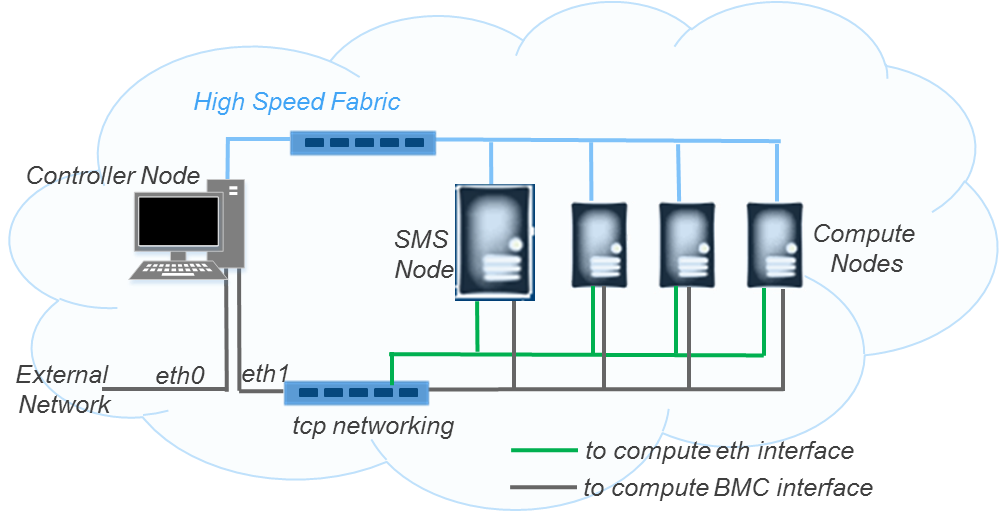
\includegraphics[width=0.85\linewidth]{HPCaaS-diagram.png}
\vspace*{-0.2cm}
\caption{Overview of physical cluster architecture.} \label{fig:physical_arch}
\end{figure}
\mbox{}

\vspace*{0.5cm}

An outline of the physical architecture discussed is shown in
Figure~\ref{fig:physical_arch} and highlights the high-level networking
configuration. The {\em controller} and {\em sms} hosts require at least two Ethernet interfaces with {\em eth0} connected to the local data center network and {\em eth1} used to provision and manage the cluster backend (note that these interface names are examples and may be different depending on local settings and OS conventions). Two logical IP interfaces are expected to each compute node: the first is the standard Ethernet interface that will be used for provisioning and resource management. The second is used to connect to each host's BMC and is used for power management and remote console access. Physical connectivity for these two logical IP networks is often accommodated via separate cabling and switching infrastructure; however, an alternate configuration can also be accommodated via the use of a shared NIC, which runs a packet filter to divert management packets between the host and BMC.

 In addition to the IP networking, there is a high-speed network
(\InfiniBand{} in this recipe) that is also connected to each of the
hosts. This high speed network is used for application message passing and
optionally for \Lustre{} connectivity as well. The high-speed network, though not required, provides higher HPC application performance (higher throughput) compare to an ethernet only system.

NOTE: This recipe sets various environment variables in one section and uses them in other sections. Users are expected to use single shell session for successful execution of this recipe. 

%Appendix A provides reference to pre-built recipe, and useful for users who wants to try out with minimum human interactions.

